\documentclass{ctexart}
\usepackage{graphicx}
\usepackage{caption}
\usepackage{float}
\usepackage{amsmath}
\usepackage{fancyhdr}
\usepackage{xunicode-addon}
\usepackage{booktabs}
\usepackage[a4paper,hmargin=1.25in,vmargin=1in]{geometry}
% !TeX program = xelatex
\title{\begin{figure}[H]
	\centering 
	\includegraphics[height=7cm,width=14cm]{E:/Pictures/中科大.jpg}
	\end{figure}\Huge\textbf{Lab 3}\\\huge{}}
\date{}
\punctstyle{banjiao} 
\pagestyle{fancy}
	\fancyhead[C]{\LARGE\textbf{Report 3}}
	\fancyhead[L]{}
	\fancyhead[R]{}
	\fancyfoot[C]{\thepage}
\begin{document}
	\maketitle
	\thispagestyle{empty}
	
	\[\makebox{\Large{姓名:\underline{\makebox[5cm]{高茂航}}}}\]
	
    \[\makebox{\Large{学号:\underline{\makebox[5cm]{PB22061161}}}}\]
	
	$$\makebox{\Large{日期:\underline{\makebox[5cm]{2024.4.28}}}}$$
	
	\clearpage

	\pagenumbering{arabic}
    \section{Task1}
    \subsection{Algorithm Description}
	

本节主要是调用了pandas库,对数据进行一系列处理,
包括读取数据、查看数据的前10行、查看数据的信息、
删除缺失值、重置索引、删除id列、查看diagnosis列的值的个数、
将diagnosis列的值转换为0和1、查看2-7列的统计信息、查看不同diagnosis值的各组数据所有特征的变异系数,详情在代码文件中显示。
\subsection{Results}
\begin{figure}[H]
	\centering 
	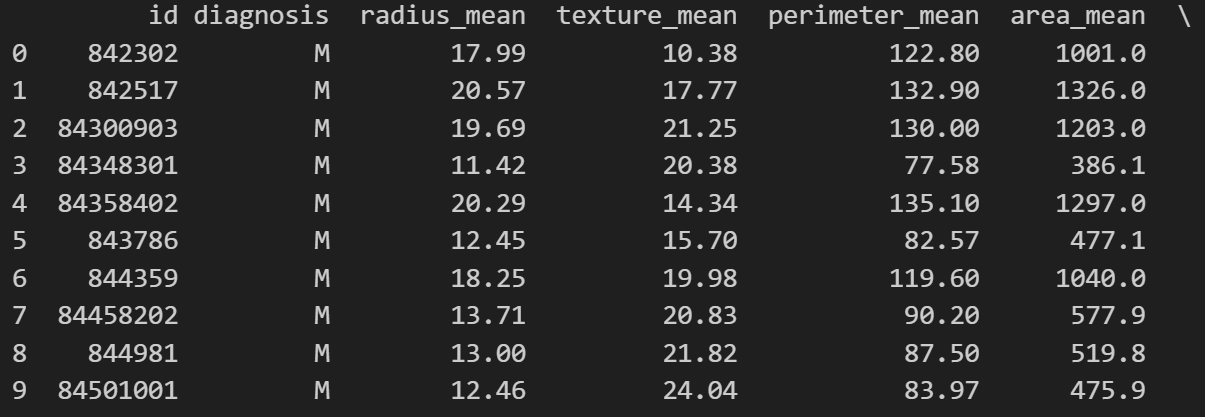
\includegraphics[height=5cm,width=14cm]{1.png}
	\end{figure}
	\begin{figure}[H]
		\centering 
		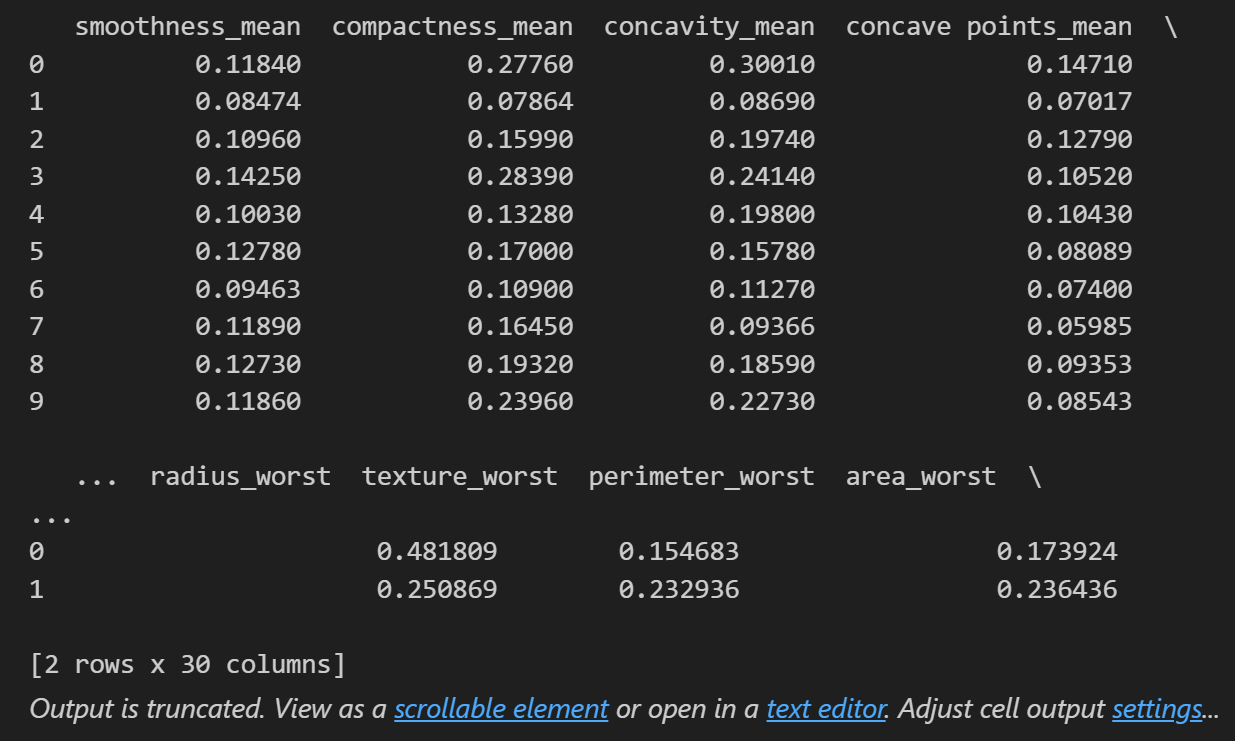
\includegraphics[height=8cm,width=14cm]{2.png}
		\end{figure}
		限于篇幅,没将Task1的全部结果显示出来。
    \section{Task2}
    \subsection{Algorithm Description}
	
	本节调用了numpy和matplotlib库,对数据进行一系列处理,如
	绘制频率分布直方图、绘制分布散点图、corr()求Pearson相关系数矩阵、用matshow(corr, cmap='coolwarm')绘制相应
	的相关系数热力矩阵图等,由于都是固定的操作,故不再详述代码细节。
\subsection{Results}
\begin{figure}[H]
	\centering 
	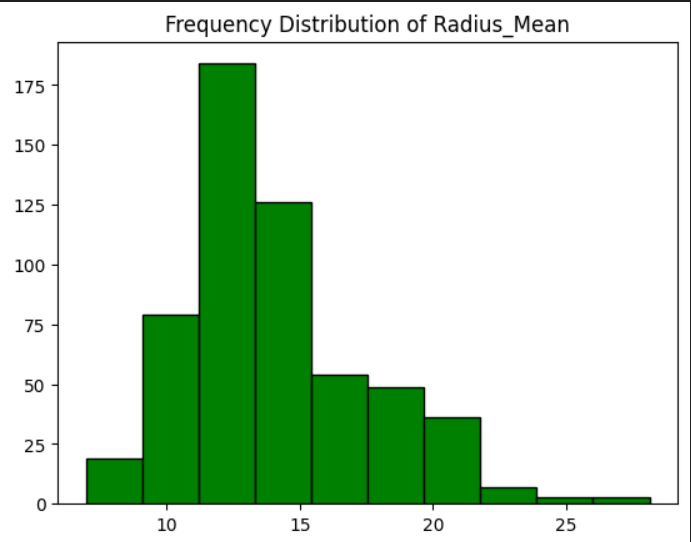
\includegraphics[height=9cm,width=14cm]{3.png}
	\end{figure}
	\begin{figure}[H]
		\centering 
		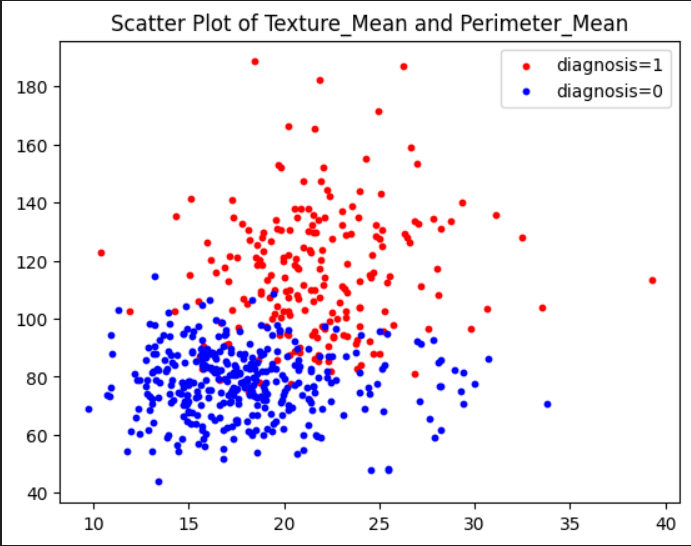
\includegraphics[height=9cm,width=14cm]{4.png}
		\begin{figure}[H]
			\centering 
			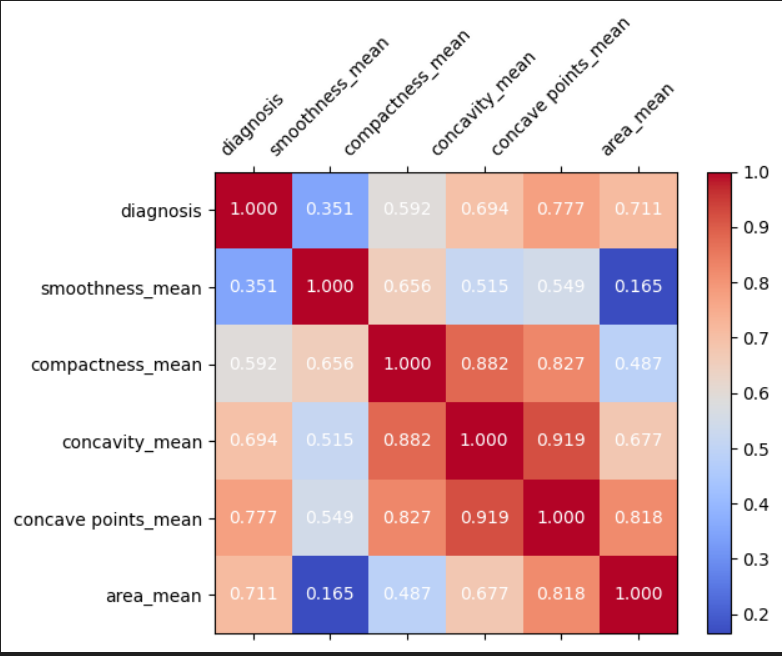
\includegraphics[height=10cm,width=14cm]{5.png}
			\end{figure}
		\end{figure}
    \section{Task3}
    \subsection{Algorithm Description}
	先用np.column\_stack()将三个一维数组堆叠成一个二维数组,每个一维数组成为新二维数组的一列,
	进而代入公式求最小二乘估计,再使用numpy.polyfit()方法做二次多项式拟合,并绘制拟合曲线,可以发现数据适合二次函数拟合,而不适合线性拟合。
\subsection{Results}
\begin{figure}[H]
	\centering 
	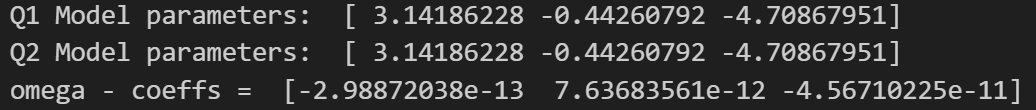
\includegraphics[height=1.5cm,width=14cm]{6.png}
	\end{figure}
	\begin{figure}[H]
		\centering 
		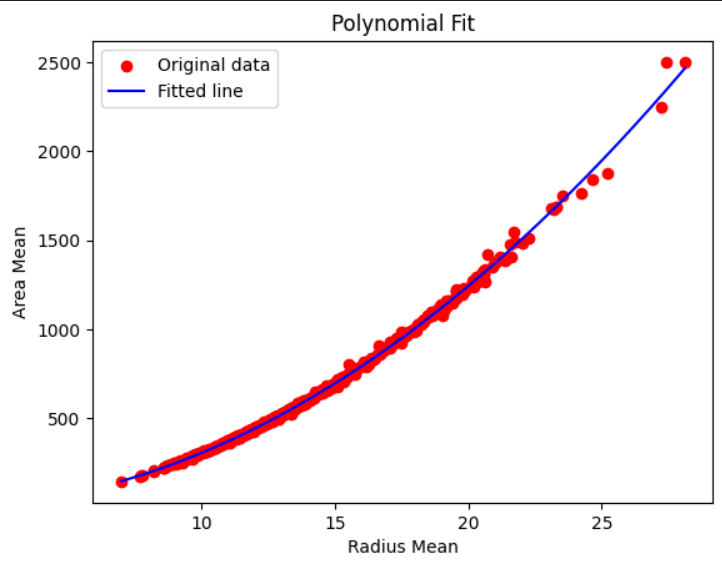
\includegraphics[height=9cm,width=14cm]{7.png}
		\end{figure}
    \section{Task4}

	\subsection{Algorithm Description}
	利用numpy.cov()和numpy.linalg.eig()求X的协方差矩阵corX,进而求corX的特
征值eigV与特征向量矩阵eigMat,通过计算验证eigMat的正交性,接着对X进行PCA,得到Z,可以发现Z的数据的纵坐标基本在0附近,
即PCA将X的数据映射到接近一维空间上。也能发现cov(Z)的对角元与eigV的值相等,且非对角元十分接近于0。
删除Z的一维数据,即可完
成主成分分析降维过程。


	\subsection{Results}
	\begin{figure}[H]
		\centering 
		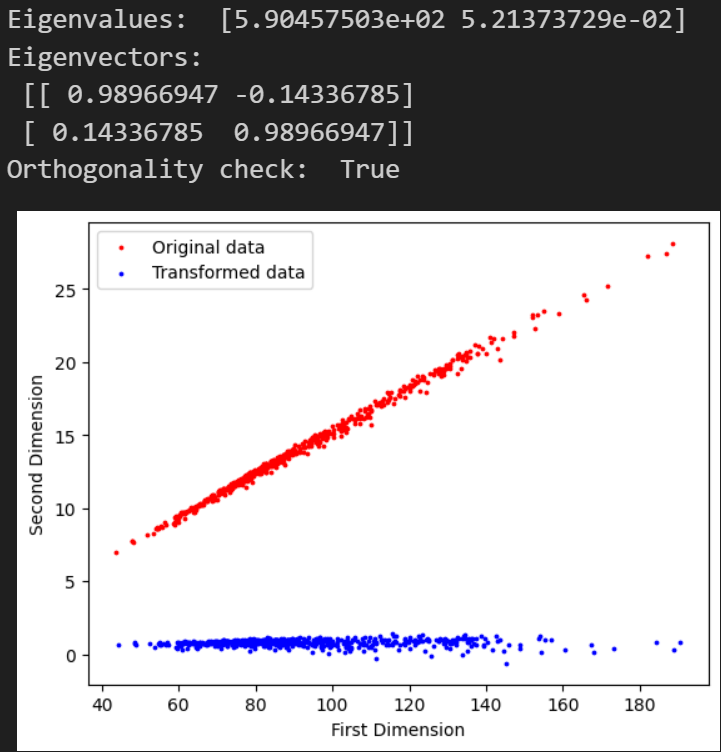
\includegraphics[height=12cm,width=14cm]{8.png}
		\end{figure}
		\begin{figure}[H]
			\centering 
			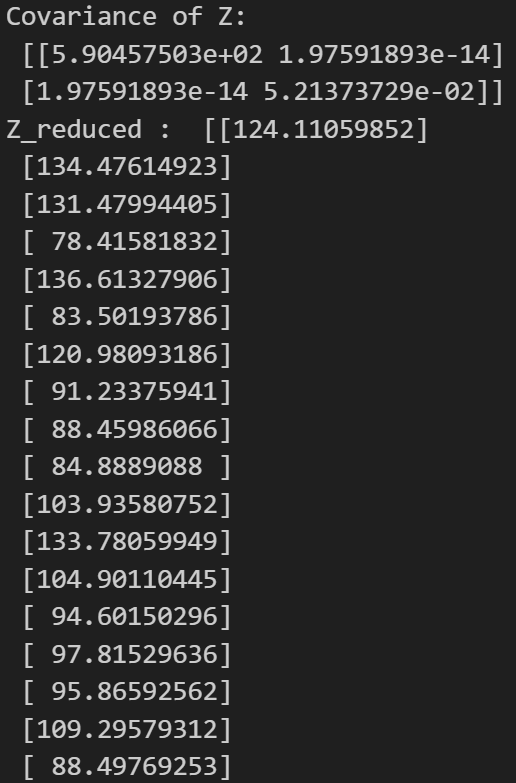
\includegraphics[height=8cm,width=5cm]{9.png}
			\end{figure}
		限于篇幅,没将Z\_reduced的全部结果显示出来。
	\section{Task5}

	\subsection{Algorithm Description}
	本情景应该进行成组检验,因为两组数据相互独立,
	单侧检验原假设为Mean of group1 = Mean of group2。
	因为p值为5.469799049160595e-56远小于0.05,因此很有把握否认原假设,接受备择假设,即Mean of group1 <= Mean of group2。
\subsection{Results}
\begin{figure}[H]
	\centering 
	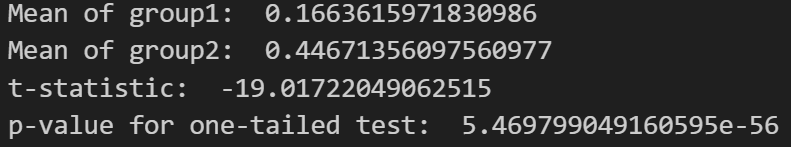
\includegraphics[height=1.5cm,width=8cm]{10.png}
	\end{figure}

\end{document}